\documentclass{standalone}
\usepackage[T1]{fontenc}
\usepackage{siunitx}
\usepackage{tikz}

\usetikzlibrary[arrows,positioning,matrix]

\begin{document}
\begin{tikzpicture}
  \node[draw=none] (topleft) {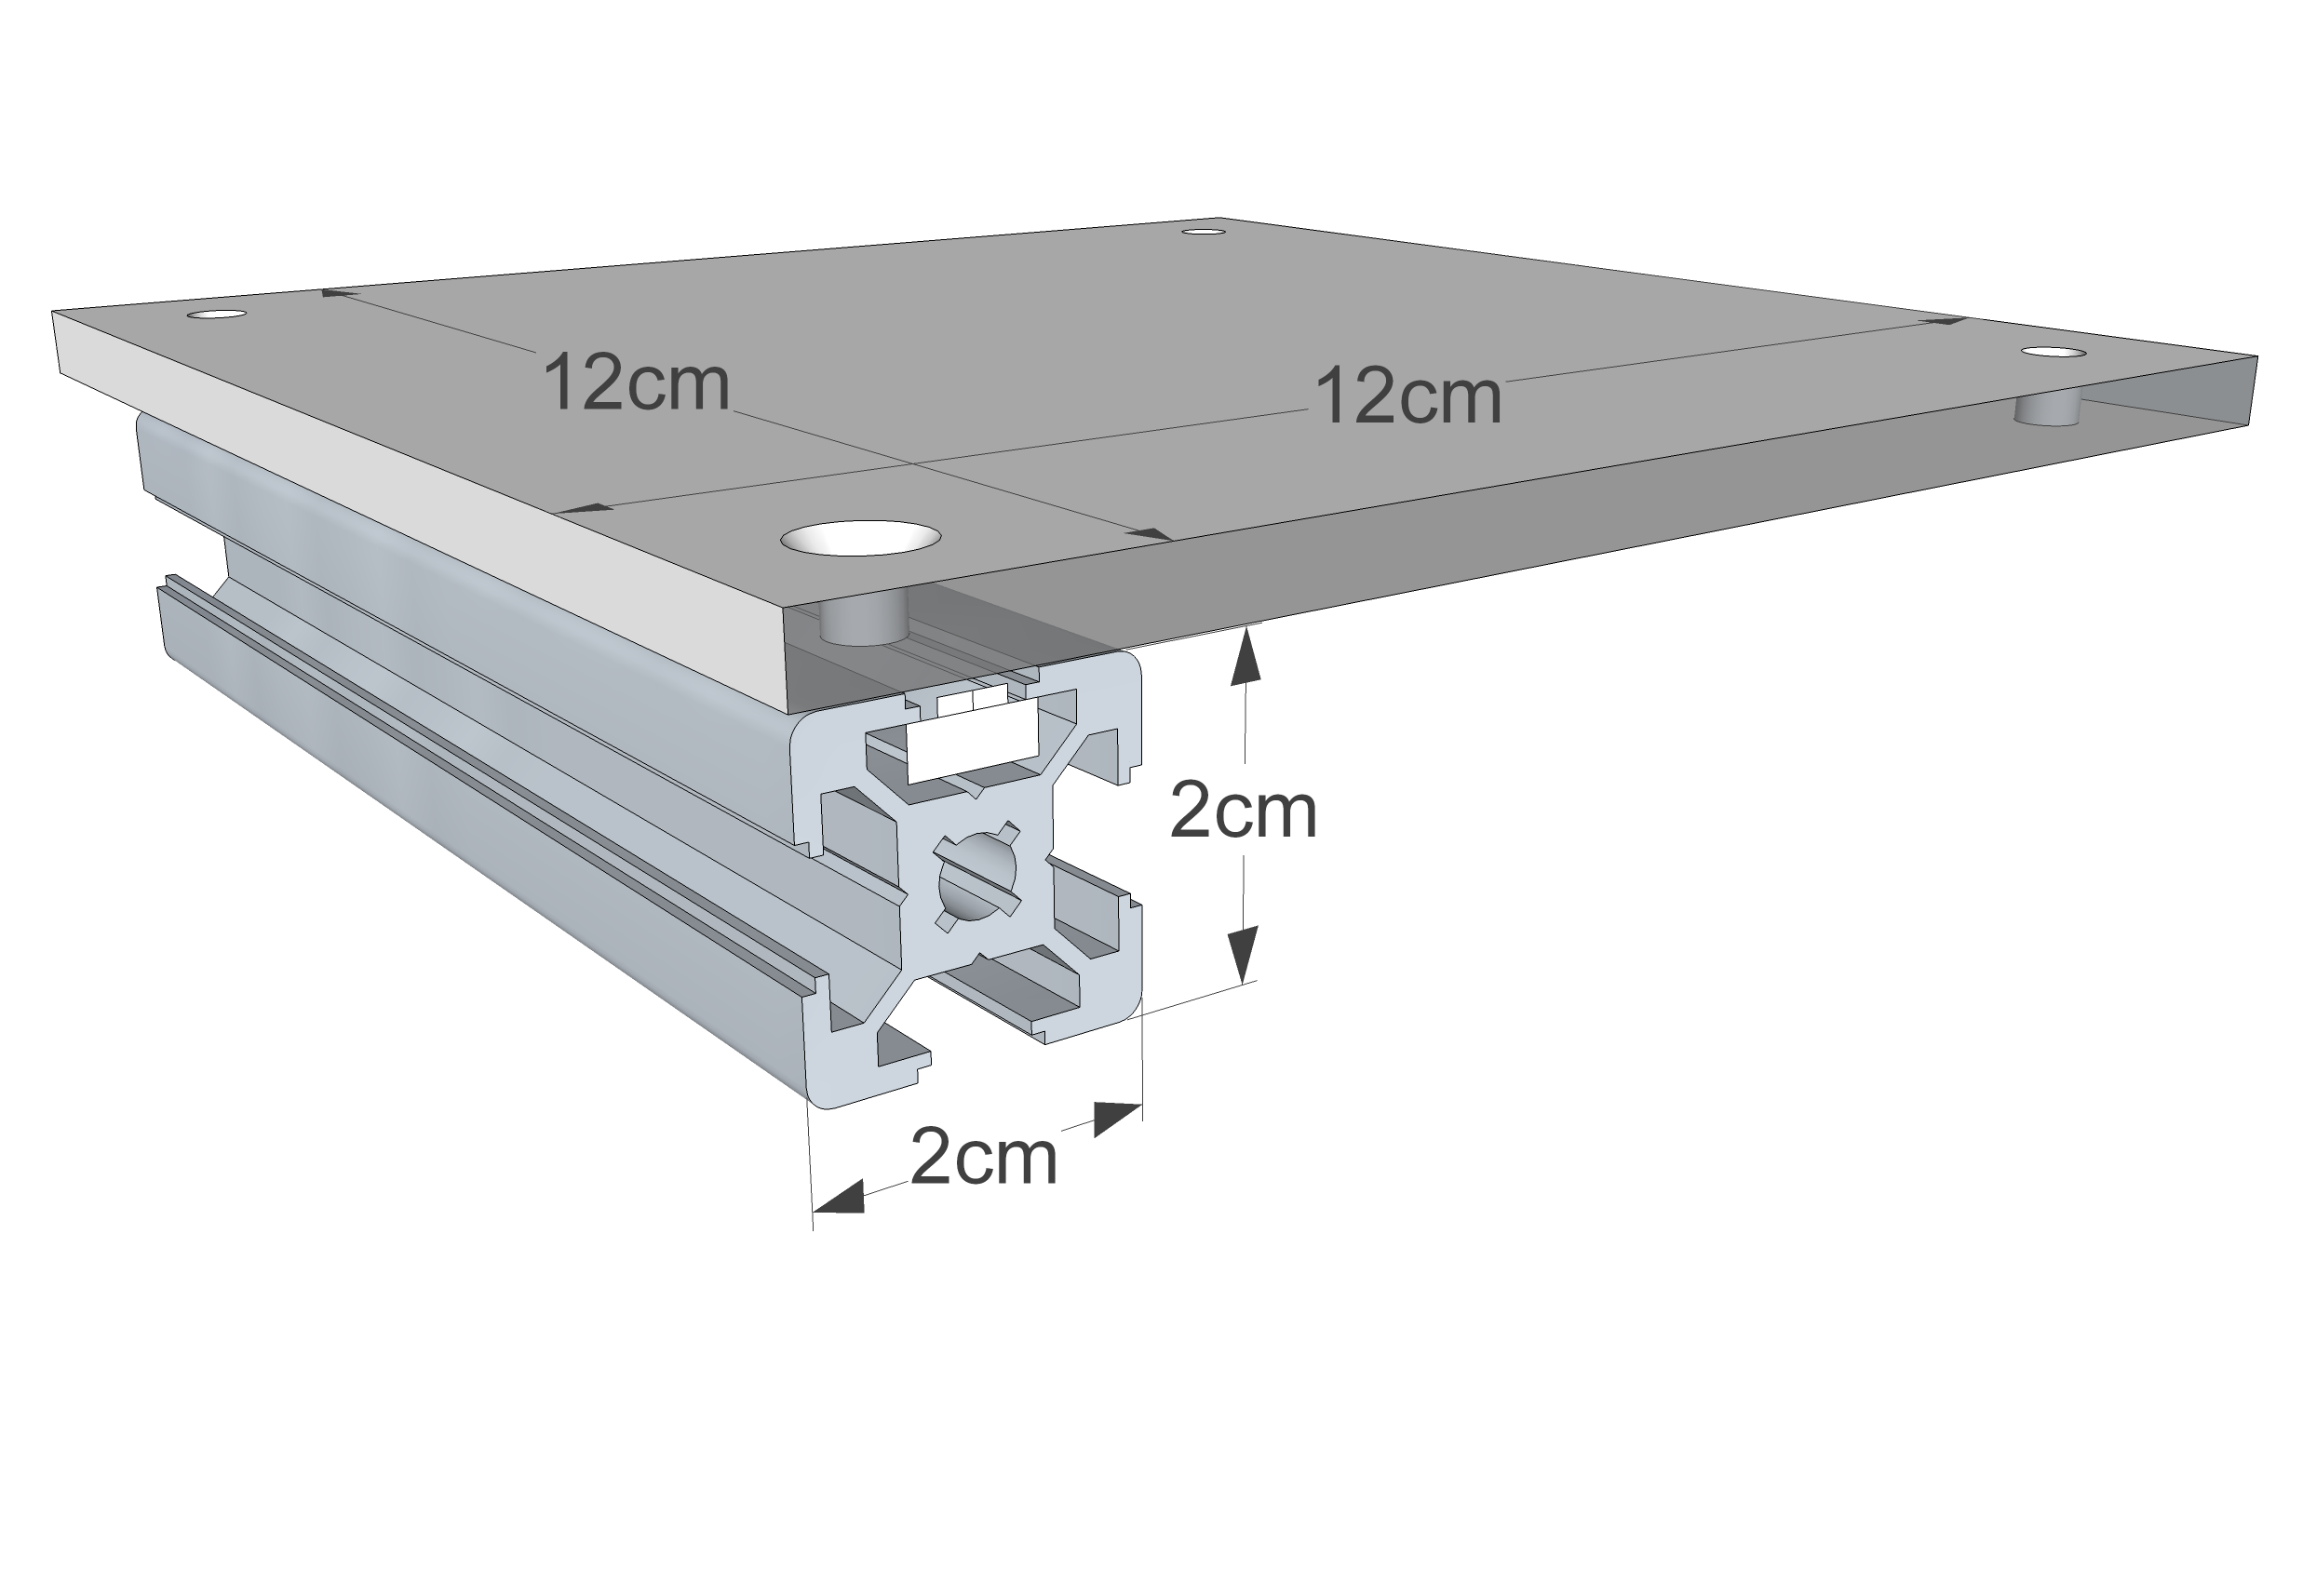
\includegraphics[width=0.5\textwidth]{elements/1x1_module}};
  \node[draw=none,above left=0mm of topleft] {A};
  \node[draw=none,below right=-5.4cm and 3.5mm of topleft] (volumes) {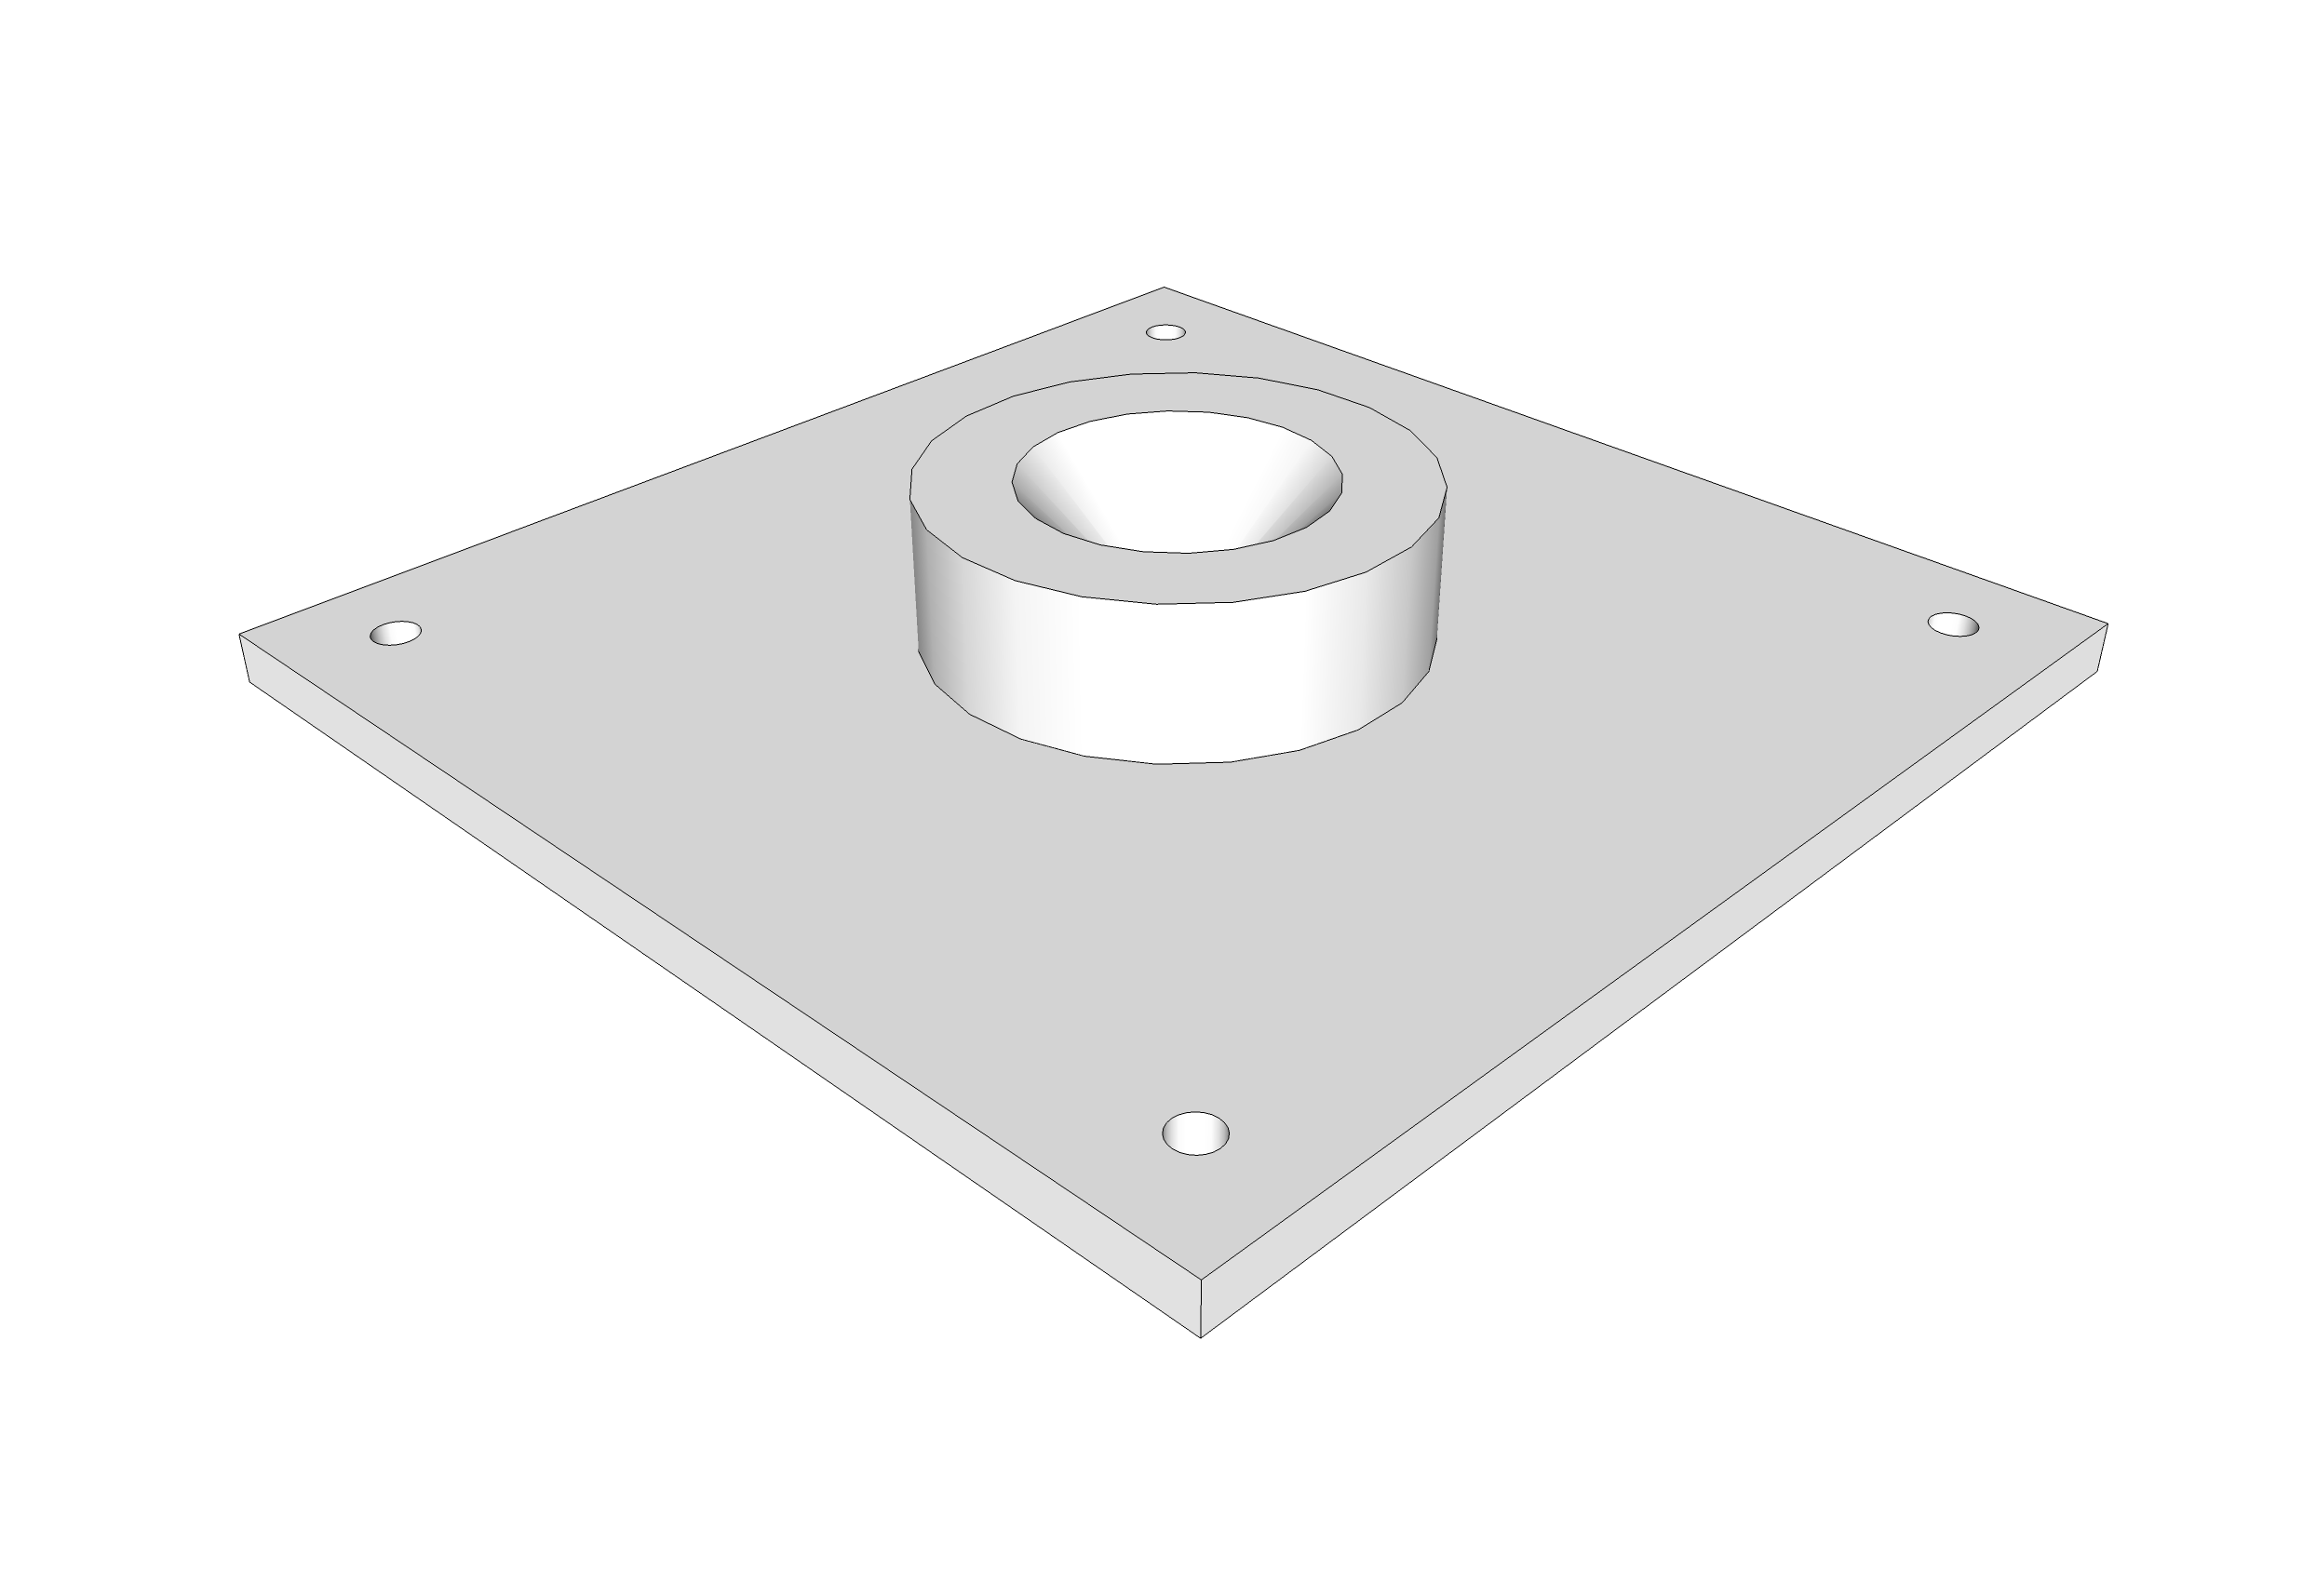
\includegraphics[width=0.5\textwidth]{elements/1x1_poke_module}};
  \node[draw=none,above right=0mm and 2mm of topleft] {B};
  \node[draw=none,below=-0.5cm of topleft] (bottomleft) {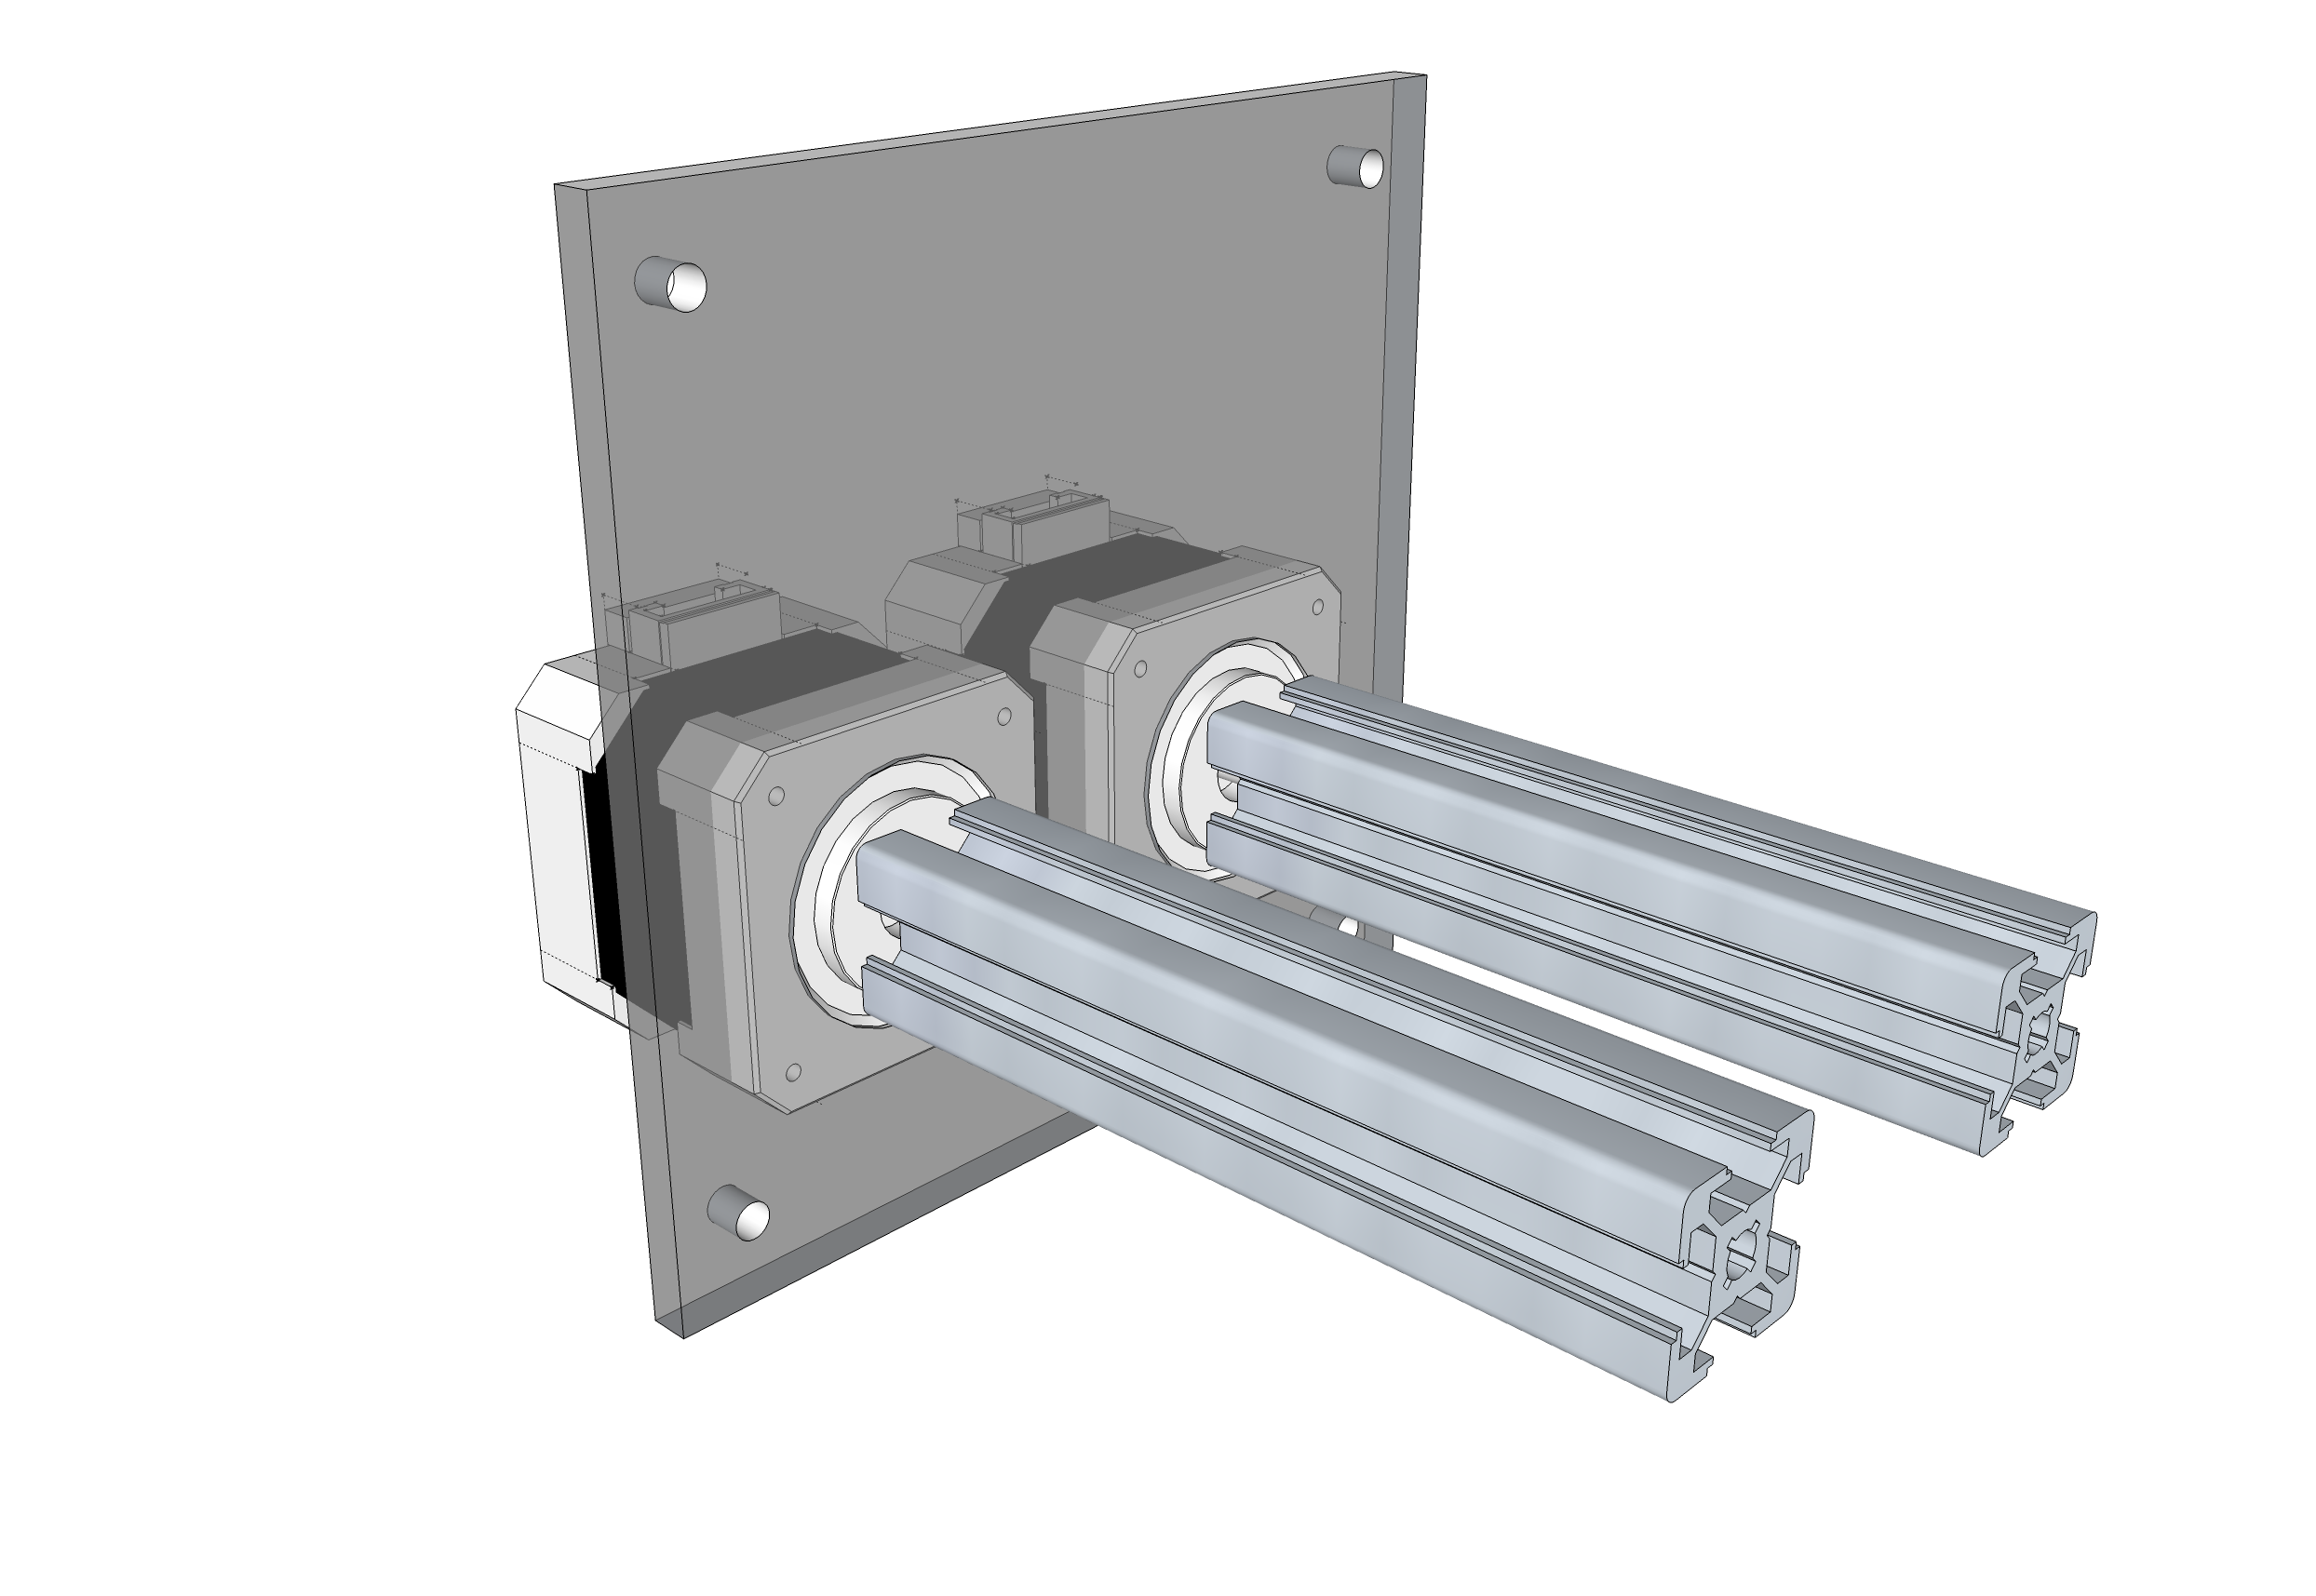
\includegraphics[width=0.5\textwidth]{elements/1x1_stepper_module_translucent}};
  \node[draw=none,above left=-5mm and 0mm of bottomleft] {C};
  \node[draw=none,right=of bottomleft] (bottomright) {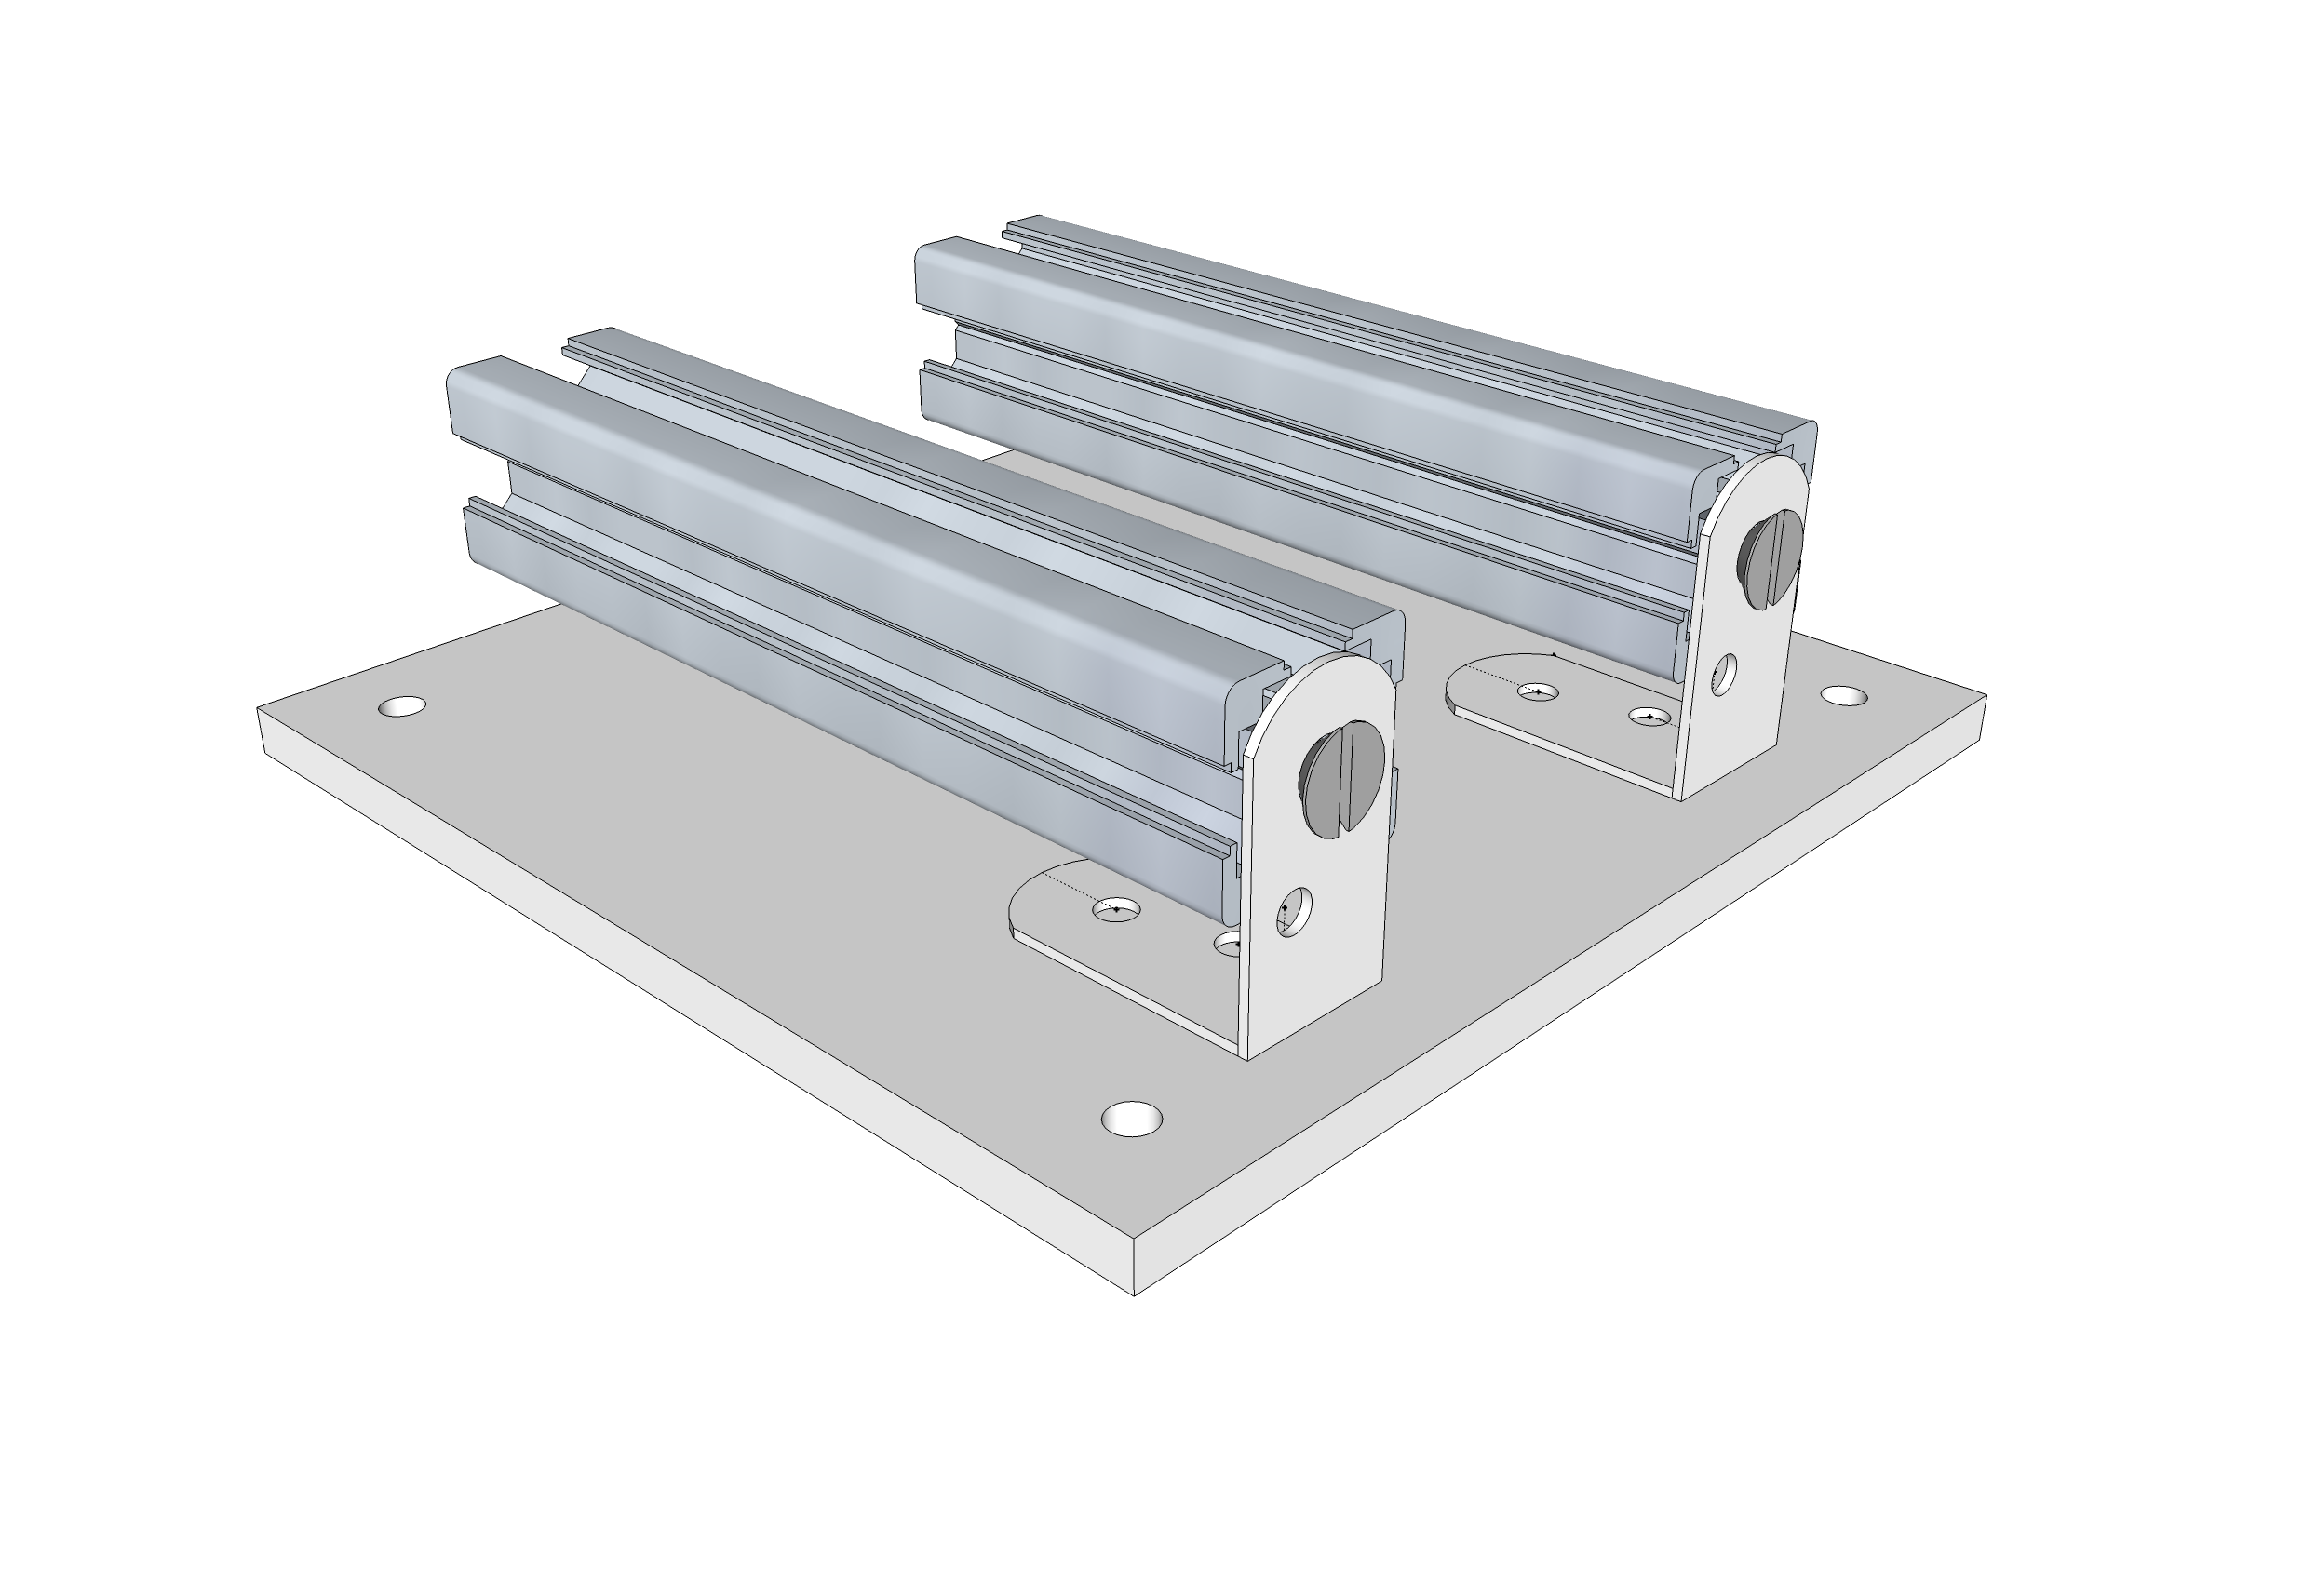
\includegraphics[width=0.5\textwidth]{elements/1x1_step_module}};
  \node[draw=none,above left=-5mm and 0mm of bottomright] {D};
\end{tikzpicture}
\end{document}